\chapter{Introduction}
\label{ch.intro}

	% Context
	% Historical background
	% Frequency barrier
	For several years, the increase in the frequency of processors was
	employed as the main technique for achieving performance
	improvements. However, as a side effect, the temperature of
	processors started rising to high values, thus imposing a physical
	limit to the aforementioned technique. Alternatively, the constant
	improvement of semiconductor technology helped to mitigate the
	impact of this problem, allowing the industry to build more powerful
	processors with the same frequency. Therefore, knowing the
	frequency barrier and the imminent end of Moore's
	Law~\cite{moore:1965}, the academy and industry began to research
	and invest in alternatives to keep increasing the processing power
	of computer systems.

	% Improves architectural parts
	\autoref{fig:microprocessor-data} illustrates the paradigm shift
	that processors have gone through to the present day. From mid-2000,
	the frequency of processors tended to stagnate. The steady increase
	in transistors in the same chip area and the vast diversity of
	trade-offs to improve single-thread performance has softened the
	frequency impact on processors. Some significant trade-offs are
	different types of instruction sets, instruction parallelism,
	out-of-order processing techniques, branch prediction techniques,
	and various memory hierarchies. Then, in mid-2005, the performance
	of computer systems was pushed even further by increasing the number
	of processing cores in a single die. These architectures, called
	\textit{multicores}, allowed the continuous rise of the computing
	performance.

	The ever-increasing number of transistors and cores in a chip
	quickly led to the advent of \manycores. Notwithstanding, the line
	between \textit{multicores} and \manycores is very tenuous. Some
	researchers argue that in the latter architectures, losing a core it
	will not significantly impact the performance of the platform. A
	system is classified as \manycore when there is a need for
	distributed memory and on-chip networking~\cite{freitas:thesis}.

	\begin{figure}[t]
		\centering%
		\caption{Multiprocessor evolution.}%
		\label{fig:microprocessor-data}%
		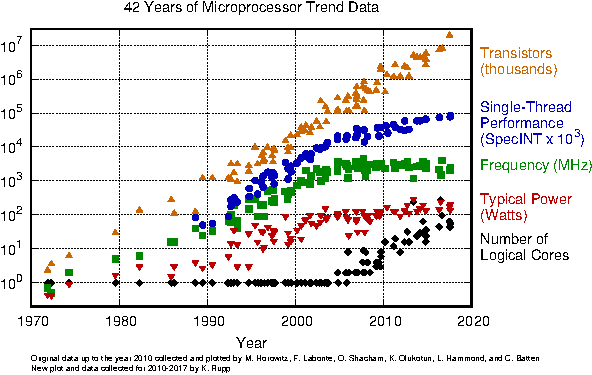
\includegraphics[width=.85\textwidth]{42-years-processor-trend.pdf}%
		\fonte{Adapted from \citeonline{url:microprocessor-trend-data}.}%
	\end{figure}

	% From multicore to manycores and Manycores characteristics
	Yet another classification for manycores is based on
	their ratio between processing speed, measured by the number of \flops, and power consumption,
	in \watts. \autoref{fig:microprocessor-data} pictures that even as the
	number of cores increasing, typical power has not grown uncontrollably.
	For instance, to achieve \exascale ($10^{18}$ \flops), the US Department
	of Defense issued a report stipulating the energy efficiency of a
	supercomputer should be around 50 GFLOPS/\watts~\cite{darpa:exascale}. 
	To cope with this energy constraint, a new class of
	parallel processors, called \textit{\lightweight \manycores}, emerged to
	provide high parallelism with low power consumption.
	Lightweight manycores differ from traditional large-scale
	multicores and manycores in several points: 

	\begin{itemize}
		\item They integrate thousands of low-power cores in a single die organized in clusters;
		\item They are designed to cope with \mimd workloads;
		\item They rely on a high-bandwidth \noc for fast and reliable message-passing communication;
		\item They have constrained memory systems; and
		\item They frequently feature a heterogeneous configuration.
	\end{itemize}

	Some industry-successful examples of \lightweight \manycores are the
	\mppa~\cite{DeDinechin2013-1}; the \epiphany~\cite{olofsson2014};
	and the \taihulight~\cite{zheng2015}. Together with superior performance
	scalability and energy efficiency, lightweight manycores brought a new
	set of challenges in software development coming from their
	architectural particularities. More precisely, these 
	introduced the following difficulties:

	\begin{itemize}
		\item \textit{Hybrid programming model:} due to the parallel and
		distributed nature of the architecture, engineers are frequently
		required to adopt a message-passing programming model to deal
		with the presence of rich \nocs~\cite{kelly2013} that
		interconnects clusters and a shared-memory model inside the
		cluster;

		\item \textit{Missing hardware support for cache coherency:} to
		reduce power consumption, theses processors do not feature cache
		coherency, which in turn forces programmers to handle it
		explicitly in software level and frequently calls out for a
		redesign in their applications~\cite{francesquini2015};

		\item \textit{Constrained memory system:} the frequent presence
		of multiple physical address spaces and small local memories
		require data tiling and prefetching to be handled by the
		software~\cite{Castro2016};

		\item \textit{Heterogeneous configuration:} the different
		programmable components on \lightweight \manycores turns the
		actual deployment of applications in a complex
		task~\cite{barbalace2015}.
	\end{itemize}

	% Challenges and Problem Definition
	Part of these challenges derives from existing runtimes and \oss.
	On the one hand, runtimes do not hide the characteristics of hardware
	making software development more challenging and non-portable, \eg they
	neither allow direct access to non-local data, nor the manipulation of
	them in a transparent way. Thus, fundamental \os mechanisms, such
	as core multiplexing, core partitioning, and process and data
	migration, may not be addressed. On the other hand, the complicated
	portability and scalability of traditional \oss with monolithic
	kernels, which were designed to homogeneous hardware, is leading to
	alternative \os designs~\cite{Baumann2009, kluge2014, nightingale2009, rhoden2011}.

	% Goals and Contributions
	We believe that \oss for the next-generation of \lightweight
	\manycores must be redesigned from scratch to cope with their tight
	architectural constraints. Based on this idea, a new fully-featured
	distributed \os based on a multikernel approach~\cite{Baumann2009}
	is under investigations~\cite{penna2017-1,penna2017-2,penna2019}.
	The \textit{\nanvixmultikernel} features a generic and flexible \hal for
	\lightweight \manycores that addresses the key issues encountered in
	the development for these processors. On top of the \textit{Nanvix \hal},
	a microkernel is being designed and implemented to provide the bare bones
	of the most important system abstractions.

\section{Goals}
\label{sec.goals}

	Based on the aforementioned motivations, the primary and specific
	goals of this work are detailed next.

\subsection{Main Goal}
\label{sec.goals.main}

	The main goal of this undergraduate dissertation is to propose an
	\textit{Inter-Cluster Communication Module} to the \textit{\nanvixhal}
	and port it to the \mppa manycore processor~\cite{DeDinechin2013-1}.
	This module exposes the essential abstractions that allow overlying
	layers to create richer communication services. Using this module, we
	also propose \textit{Inter-Cluster Communication Services} to the
	\textit{\nanvixmicrokernel}. This work is part of the collaborative
	project between \ufsc, \pucminas, and \uga to develop an \os for
	\lightweight \manycore platforms.

\subsection{Specific Goals}
\label{sec.goals.specific}

	\begin{itemize}
		\item Definition and proposal of an \textit{Inter-Cluster Communication Interface} for lightweight manycores;

		\item Implementation of the proposed interface in the \textit{\nanvixhal} for the \mppa lightweight manycore processor;
		
		\item Integration of the \nanvixhal interface with the \textit{\nanvixmicrokernel};
		
		\item Performance evaluation of \nanvixmicrokernel implementation using synthetic micro-benchmarks that reproduce the \textit{collective communication routines} of the \mpi programming model.
	\end{itemize}

\section{Organization Of The Work}
\label{sec.organization}

	The remainder of this work is organized as follows.
	In \autoref{ch.background}, we present a background on \os and communication
	design for multicores and multicomputers, the MPPA-256 lightweight manycore
	processor and the Nanvix project.
	In \autoref{ch.related-work}, we discuss the principal related work.
	In \autoref{ch.development}, we discuss the design and implementation
	of the inter-cluster communication facility.
	In \autoref{ch.experiments}, we detail the evaluation methodology
	that we adopted and analyze our experimental results.
	Finally, in \autoref{ch.conclusions}, we draw our conclusions and future work.
